\subsection{Taylor-Couette Flow}

\begin{figure}[!bp]
  \begin{minipage}[c]{0.6\textwidth}
      \centering
        \resizebox{0.9 \textwidth}{!}{
       \import{gfx/immersed_boundary/tcflow//}{tcsystem.pdf_tex}
      }
  \end{minipage}
  \begin{minipage}[c]{0.3\textwidth}
      \caption{Taylor-Couette test case. Two cylinders with radii $r_i$ and $r_o$ and angular velocities $\Omega_i$ and $\Omega_o$ are oriented coaxial and parallel to the
      $z$ axis.
      \label{validation:setup_tcflow}
      }
  \end{minipage}
\end{figure}

The setup of the Taylor-Couette flow test case is shown in Fig. \ref{validation:setup_tcflow}.
It contains of two coaxial cylinders which are oriented parallel to the z-axis.
The inner cylinder has a radius and angular velocity $r_i$ and $\Omega_i$, in analogy we define
$r_o$ and $\Omega_o$ for the outer cylinder.
The fluid domain is given by the gap of width $d = r_o - r_i$ between the cylinder and extends to infinite.
For the simulation  periodic boundaries are used in $z$-direction.

In constrast to the previously examined test cases this system provides different characteristics
of the flow regime at the immersed boundaries. The flow along the boundary is not orthogonal to the curvature of the geometry,
Furthermore the velocity at the boundarys is not zero, the boundarie needs to fullfill the Dirichlet condition, which is given by
$|\vec{v}(\vec{r})|_{r_i} | = |\Omega_i \times \vec{r}|$.

In dependency of the domain paratemers different flow regimes can occur.
For small differences in the rotation rate the flow is laminar and azimuthal.
An increase of the angular velocity of the inner cylinder leads to an instability.
In this flow regime toroidally vortices form, which are also denoted as Taylor cells,
the flow is not pure azimuthal \citep{tritton88}.
In this testcase only the laminar and azimuthal flow regime, where the outer cyinder is not rotating ($\Omega_o = 0$), will be considered.
In literature this system is usually referred to as circular coutte flow (CCF) \citep{Kundu2012}.

The problem can be reduced to polar coordinates $(r, \phi)$ and the equations of motion for the steady state are given by \citep{Kundu2012}
\begin{align}
    \label{vali:tc_flow_eqnavstok}
    -\frac{v^2_\phi}{r} = - \frac{\partial p}{\partial r} \qquad ;& \qquad 0 = \frac{1}{Re}\frac{\partial}{\partial r}\left(\frac{1}{r}\frac{\partial}{\partial r}(r v_\phi)\right)
\end{align}

\clearpage

For the non-dimensionalization we choose the default convention, according to  \citep{Chen2015}
\begin{align}
    \text{Length:}\qquad &  \vec{r}^* = \frac{\vec{r}}{r_o - r_i}  &
    \qquad \text{Velocity:}\qquad& \vec{v}^* =  \frac{\vec{v}}{r_i\Omega_i}\\
    \text{Time:}  \qquad & t^* = t \cdot \frac{r_i \Omega_i}{r_o - r_i}&
    \qquad  \text{Pressure:}\qquad & p^* = \frac{\nabla p_\infty}{r_i^2\Omega_i^2}
\end{align}


The flow is then characterized by the Reynolds number $Re = \nicefrac{\Omega R_1d}{\nu}$.
With the integration of Eq. \ref{vali:tc_flow_eqnavstok}, according to \citep{Kundu2012}, the solution is given by
\begin{align}
    v_\phi = Ar + \frac{B}{r}
\end{align}
where $A$ and $B$ are defined as
\begin{align}
    A := \frac{-\Omega_i r_i^2}{r^2_o - r^2_i} \qquad ;& \qquad B := \frac{\Omega_i r^2_i r^2_o}{r^2_o - r^2_i}
\end{align}

\subsection{Simulations}


The simulations for this testcase were carried out in analogy to the Hagen-Poiseuill flow, see Sec. \ref{vali:hpflow_simsetups}.
Here the resolution is varied on the $x$ and $y$ axis, the radii are set to $r_i=1$ and $r_o=2$ and $l_x=l_y=2.5$.
The main parameters of the grid convergence study simulation are  given by

\begin{center}
\vspace*{0.7ex}
\begin{tabular}{c|c|c|c|c|c|c|c }
 $ N  $                   & $\Delta t$ & $\Delta z$            & $\Rey$  & $c^2$   & $l_x, l_y$ & $r_o, r_i$ & $T_{end}$\\
\hline
 $512, [16, 256], \Delta N = 16 $& $10^{-4}$ & $\nicefrac{1}{N}$ & 500     & $500$   & (2.5, 2.5) & (2, 1)     & 20\\
\end{tabular}
\vspace*{0.7ex}
\end{center}

The main parameters of the long-term simulations are  given by

\begin{center}
\vspace*{0.7ex}
\begin{tabular}{c|c|c|c|c|c|c|c }
 $ N  $                   & $\Delta t$ & $\Delta x$            & $\Rey$  & $c^2$   & $l_x, l_y$ &$r_o, r_i$ & $T_{end}$\\
\hline
 $96 $& $10^{-4}$ & $\nicefrac{1}{N}$ & 500     & $500$   & (2.5, 2.5)  & (2, 1)    & 10\\
\end{tabular}
\vspace*{0.7ex}
\end{center}

\clearpage

\subsection{Results}

\subsubsection{Grid Convergence Study}


The results of the grid convergence study are shown from Fig. \ref{vali:tc_flow_gc_vp} to Fig. \ref{vali:tc_flow_gc_all}.
For a better overview the results are distributed into four plots.

In Fig. \ref{vali:tc_flow_gc_vp} the relative $l_2$-error is shown for different VP-methods.
For the VP-FD2 method the error convergence rate is about $\lambda=1.07$,
for the VP-FD4 method about $\lambda=1.16$, however it can be seen that the convergence decreases above $N\approx100$.
In this interall the error of the VP-FD4 method remains approximately constant.
The VF methods have a larger error (about $5\cdot 10^-2$ for $N=100$) in comparsion the VP methods
(between $10^{-2}$ and $2\cdot10^{-2}$.
In contrast a higher converges (about $\lambda=1.3$) can be observed for both, the FD2 and the FD4 method.

In Fig. \ref{vali:tc_flow_gc_df} the relative $l_2$-error is shown for different DF-methods.
For all methods the error convergence rate is about first order, except the DF-FD4 method which is about $\lambda=0.9$.
The smallest error is given by the DF-FD2 method which is about $\approx 2 \cdot 10^{-2}$ for $N=100$.
THis is about half an order smaller compared to the other methods.

In Fig. \ref{vali:tc_flow_gc_ip} the relative $l_2$-error is shown for different IP-methods.
For the IP-FD4 method the decay rate is about $1.47$.
For the IP-FD2 and IP+DF-FD2 method the errors are nearly  identical, the decay rate is about $1.09$
The IP+DF-FD4 method is numerically not stable and therefore not shown.
From the interpolation methods the IP-o4 method gives the smallest error for $N>100$ which is of order $10 \cdot 10^{-3}$.
Again it can be seen that the convergence decreases above $N\approx100$ for all methods.

%For all methods, except IP+DF-FD4) an approximately linear decrease in the double logarithmic space can be observed.
%In summary it can be said that the overall convergence rate of the IP-FD2-method is of one order better
%than the VP-VF and DF-VF methods. The relative error of the interpolation method ranges
%between one and two order of magnitudes below all other methods, depending on the resolution.

Finally Fig. \ref{vali:tc_flow_gc_all} shows the methods with the best convergence
rates from the different DF, VP and IP methods in one plot.
It can be noted that in this validation not alle errors are decreasing linear.
The best results are given by the interpolation methods, with small differences in the overall error
and convergence rate.

\paragraph{Velocity difference profiles}\mbox{}\\

Beside the computation of the $l_2$-error the local difference between the theoretical and numerical velocity
profile was computed, by substracting the vector fields from each other in the $(x, y)$ plane.
The results for the FD2 schemes are presented in Fig. \ref{tcflow:results_vprofiles_o2}, the profiles
for the FD4 schemes are shown in the Appendix in Fig. \ref{tcflow:results_vprofiles_o4}.
From the profiles it can be noted that for all methods the difference between the numerical and
theoretical solution are the largest at the boundarie $r_i$ of the  inner cylinder.

\clearpage
\begin{figure}[!bp]
  \begin{minipage}[c]{0.5\textwidth}
      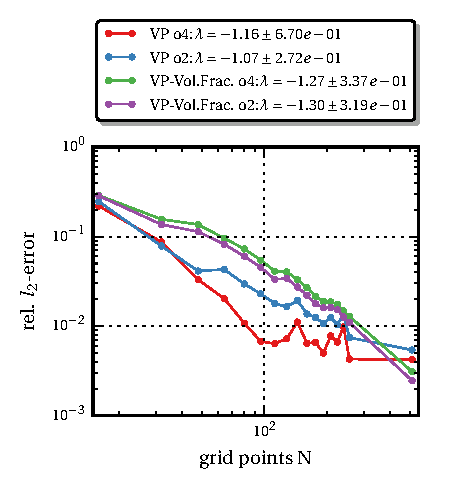
\includegraphics{gfx/immersed_boundary/tcflow/theo/vp.pdf}
      \caption{Relative $l_2$-error for different Volume-Penalization methods.}
      \label{vali:tc_flow_gc_vp}
  \end{minipage}
  \begin{minipage}[c]{0.5\textwidth}
      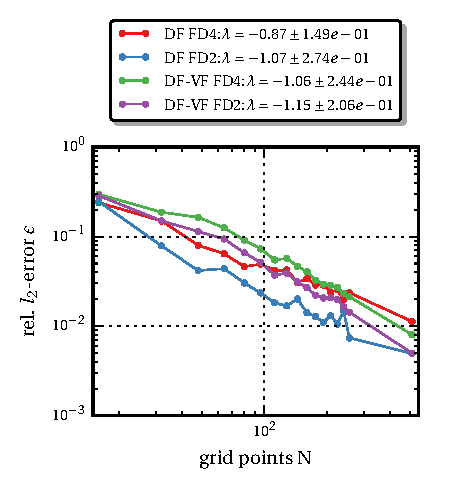
\includegraphics{gfx/immersed_boundary/tcflow/theo/df.pdf}
      \caption{Relative $l_2$-error for different Direct-Forcing methods.}
      \label{vali:tc_flow_gc_df}
  \end{minipage}
  \begin{minipage}[c]{0.5\textwidth}
      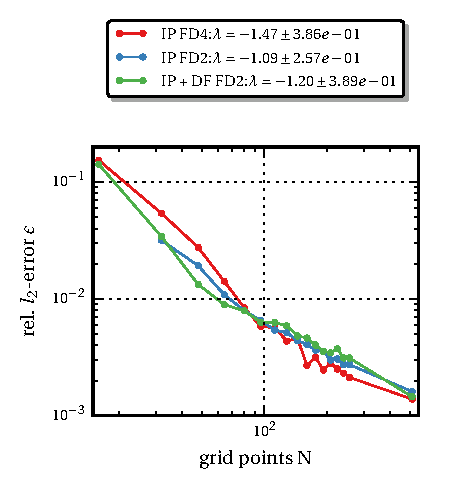
\includegraphics{gfx/immersed_boundary/tcflow/theo/ip.pdf}
      \caption{Relative $l_2$-error for different Interpolation methods.}
      \label{vali:tc_flow_gc_ip}
  \end{minipage}
  \begin{minipage}[c]{0.5\textwidth}
      \includegraphics{gfx/immersed_boundary/tcflow/theo/all.pdf}
      \caption{Relative $l_2$-error for the methods with the smallest error in comparsion.}
      \label{vali:tc_flow_gc_all}
  \end{minipage}
\end{figure}
\clearpage

\begin{figure}[!bp]
  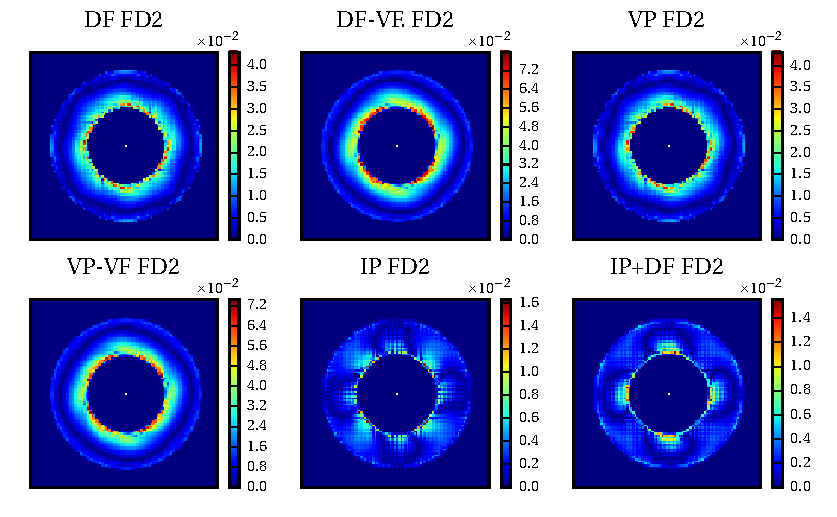
\includegraphics{gfx/immersed_boundary/tcflow/long/vz_profiles_o2.pdf}
  \caption{\label{tcflow:results_vprofiles_o2}
    Substraction of the numerial velocity profile from the theoretical
        for all FD2 methods.}
\end{figure}

\begin{figure}[!bp]
  \begin{minipage}[c]{0.5\textwidth}
      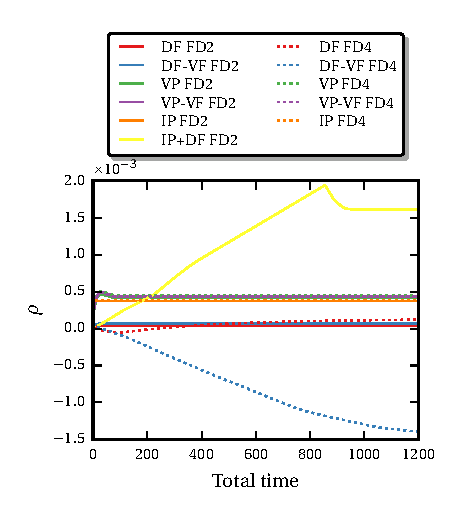
\includegraphics{gfx/immersed_boundary/tcflow/long/ts_all.pdf}
      \caption{\label{tcflow:results_long_ts_o2}
            Averaged density for FD2 metdods with respect to the simulation time.
          }
  \end{minipage}
  \begin{minipage}[c]{0.5\textwidth}
      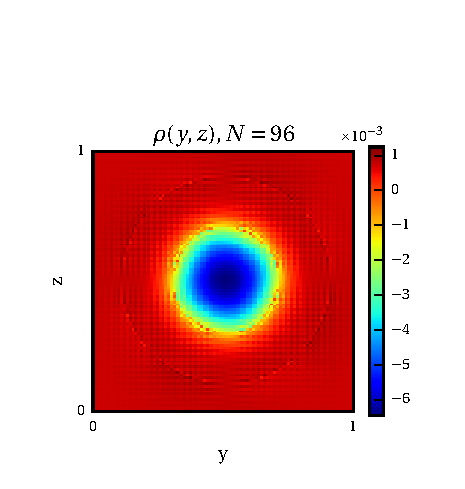
\includegraphics{gfx/immersed_boundary/tcflow/long/example.pdf}
      \caption{\label{tcflow:rho_example}
        Density oscillations for the VP-VP FD2 method.
      }
  \end{minipage}
\end{figure}

\clearpage

\subsubsection{Long-Term Simulations}

For all methods, except the IP-DF4 method, the simulations were numerically stable.
The density was averaged over the fluid domain by Eq.  \ref{vali:density_calc},
the results of the computation are shown in Fig. \ref{tcflow:results_long_ts_o2}.
For the IP+DF FD2 method the density increase until a saturation is reached, about $1.6\cdot10^{-3}$ at $T\approx 1000$.
The density of the  DF-VF FD4 decreases to about $-1.4\cdot10^{-3}$ with a saturation at $T\approx1400$.
For all other methods the saturation of the density is reached faster, at $T\approx200$.
Furthermore the averaged density is smaller, in the order $10^{-4}$.

Beside the saturations in the density for both methods FD2 and FD4 numerical oscillation can be
observed, which  are similar to the Hagen-Poiseuille flow test case.
In Fig. \ref{tcflow:rho_example} these oscillations are exemplarily shown for the VP-VF FD2 method.
Beside the oscillations of order $10^{-4}$ it can be seen that in side of the inner cylinder the
density decreases to about $-6\cdot10^{-3}$, in comparison to $\approx10^{-3}$ in the fluid domain.

\subsection{Discussion}

-density div u ist nicht 0 deswegen auch fehler in o2

-comparsion to hpflow

-velocity profiles indicate that the error of the methos  comes from the inner border

-ip diff zero o2

\clearpage

\section{Summary}

In the first part of the chapter an introduction to different immersed boundary methods was given.
The volume-penalization method, adapted from  \citep{Lulff2011} uses a forcing term in form of a damping proportional to the velocities at the immersed boundary.
In case of the Direct-Forcing method, adapted from \citep{Fadlun2000} the velocity is set directly to zero.
Both methods then were extended by the Volume-Fraction method, adapted from \citep{Fadlun2000}, which computes the wall and fluid domain ratio inside a boundary
cell and uses this value as a weighting coeffient for the forcing.
Finally an interpolation method adapted from  \citep{ Gilmanov2003} was introduced. In the first step this method performs a bilinear interpolation on a  surface
between four grid points, in the second step this value is linear interpolated on the boundary cell.

In the second part of the chapter three different test cases were introduced as a validation for the immersed boundary methods.
The laminar Poiseuille flow was used as a first validation test case for the DF and VP method with the use of FD2 and FD4.
With rhe results it was possible to identify an error in the basic algorithm of the simulation.
Furthermore it could be shown that the use of a 5-Point stencil leads to discretization errors at the immersed boundaries.

In the second test case a simulation of a Hagen-Poiseuille flow was performed.
The results of this simulation pointed out possible numerical problems.
One possible problem are numerical oscillations which are eventually caused
by the decoupling of neighboor cells in the density.
Furthermore this test case shows that the use of a 5-Point stencil creates a numerical error,
which results in a large error for the IP-DF4 method.
It can be noted that using the volume fraction method  the error of the DF and VP method can be improved.
In summary all errors are approximately below the order  $10^2$ for $N>100$,
by far the smallest error was obtained with the IP-DF2 method.
All convergence rates are at least as good in a comparsion
to the results from validation test cases from literature.

The last test case was given by a Taylor-Couette system.
In comparsion to the Hagen-Poiseuille flow the  computed numerical error is larger,
up to an order for the VF methods, which perform inferior in this testcase.
In this simulation for both the FD2 and FD4 methods small pressure oscillations can be observed.
Again the assumption is that this is a result of the decoupling.
Finally the velocity profiles show that the error is the largest to the inner domai boundary $r_i$.
This could be an indicator that the immersed boundary methods in combination with the used basic implementation
are not a good choice for moving boundaries.

outlook...
- oscilllation abklären -> rhie chow -> outlook
- interpolation fehler -> was soll man sagen
- alle methoden except ip haben gleiche fehler ordnung
- fraction methdos is a little bit better
- ip ist am besten mit 2 ordnung
-the best error is interpolation



